% Options for packages loaded elsewhere
\PassOptionsToPackage{unicode}{hyperref}
\PassOptionsToPackage{hyphens}{url}
\PassOptionsToPackage{dvipsnames,svgnames,x11names}{xcolor}
%
\documentclass[
  letterpaper,
  DIV=11,
  numbers=noendperiod]{scrartcl}

\usepackage{amsmath,amssymb}
\usepackage{lmodern}
\usepackage{iftex}
\ifPDFTeX
  \usepackage[T1]{fontenc}
  \usepackage[utf8]{inputenc}
  \usepackage{textcomp} % provide euro and other symbols
\else % if luatex or xetex
  \usepackage{unicode-math}
  \defaultfontfeatures{Scale=MatchLowercase}
  \defaultfontfeatures[\rmfamily]{Ligatures=TeX,Scale=1}
\fi
% Use upquote if available, for straight quotes in verbatim environments
\IfFileExists{upquote.sty}{\usepackage{upquote}}{}
\IfFileExists{microtype.sty}{% use microtype if available
  \usepackage[]{microtype}
  \UseMicrotypeSet[protrusion]{basicmath} % disable protrusion for tt fonts
}{}
\makeatletter
\@ifundefined{KOMAClassName}{% if non-KOMA class
  \IfFileExists{parskip.sty}{%
    \usepackage{parskip}
  }{% else
    \setlength{\parindent}{0pt}
    \setlength{\parskip}{6pt plus 2pt minus 1pt}}
}{% if KOMA class
  \KOMAoptions{parskip=half}}
\makeatother
\usepackage{xcolor}
\setlength{\emergencystretch}{3em} % prevent overfull lines
\setcounter{secnumdepth}{-\maxdimen} % remove section numbering
% Make \paragraph and \subparagraph free-standing
\ifx\paragraph\undefined\else
  \let\oldparagraph\paragraph
  \renewcommand{\paragraph}[1]{\oldparagraph{#1}\mbox{}}
\fi
\ifx\subparagraph\undefined\else
  \let\oldsubparagraph\subparagraph
  \renewcommand{\subparagraph}[1]{\oldsubparagraph{#1}\mbox{}}
\fi

\usepackage{color}
\usepackage{fancyvrb}
\newcommand{\VerbBar}{|}
\newcommand{\VERB}{\Verb[commandchars=\\\{\}]}
\DefineVerbatimEnvironment{Highlighting}{Verbatim}{commandchars=\\\{\}}
% Add ',fontsize=\small' for more characters per line
\usepackage{framed}
\definecolor{shadecolor}{RGB}{241,243,245}
\newenvironment{Shaded}{\begin{snugshade}}{\end{snugshade}}
\newcommand{\AlertTok}[1]{\textcolor[rgb]{0.68,0.00,0.00}{#1}}
\newcommand{\AnnotationTok}[1]{\textcolor[rgb]{0.37,0.37,0.37}{#1}}
\newcommand{\AttributeTok}[1]{\textcolor[rgb]{0.40,0.45,0.13}{#1}}
\newcommand{\BaseNTok}[1]{\textcolor[rgb]{0.68,0.00,0.00}{#1}}
\newcommand{\BuiltInTok}[1]{\textcolor[rgb]{0.00,0.23,0.31}{#1}}
\newcommand{\CharTok}[1]{\textcolor[rgb]{0.13,0.47,0.30}{#1}}
\newcommand{\CommentTok}[1]{\textcolor[rgb]{0.37,0.37,0.37}{#1}}
\newcommand{\CommentVarTok}[1]{\textcolor[rgb]{0.37,0.37,0.37}{\textit{#1}}}
\newcommand{\ConstantTok}[1]{\textcolor[rgb]{0.56,0.35,0.01}{#1}}
\newcommand{\ControlFlowTok}[1]{\textcolor[rgb]{0.00,0.23,0.31}{#1}}
\newcommand{\DataTypeTok}[1]{\textcolor[rgb]{0.68,0.00,0.00}{#1}}
\newcommand{\DecValTok}[1]{\textcolor[rgb]{0.68,0.00,0.00}{#1}}
\newcommand{\DocumentationTok}[1]{\textcolor[rgb]{0.37,0.37,0.37}{\textit{#1}}}
\newcommand{\ErrorTok}[1]{\textcolor[rgb]{0.68,0.00,0.00}{#1}}
\newcommand{\ExtensionTok}[1]{\textcolor[rgb]{0.00,0.23,0.31}{#1}}
\newcommand{\FloatTok}[1]{\textcolor[rgb]{0.68,0.00,0.00}{#1}}
\newcommand{\FunctionTok}[1]{\textcolor[rgb]{0.28,0.35,0.67}{#1}}
\newcommand{\ImportTok}[1]{\textcolor[rgb]{0.00,0.46,0.62}{#1}}
\newcommand{\InformationTok}[1]{\textcolor[rgb]{0.37,0.37,0.37}{#1}}
\newcommand{\KeywordTok}[1]{\textcolor[rgb]{0.00,0.23,0.31}{#1}}
\newcommand{\NormalTok}[1]{\textcolor[rgb]{0.00,0.23,0.31}{#1}}
\newcommand{\OperatorTok}[1]{\textcolor[rgb]{0.37,0.37,0.37}{#1}}
\newcommand{\OtherTok}[1]{\textcolor[rgb]{0.00,0.23,0.31}{#1}}
\newcommand{\PreprocessorTok}[1]{\textcolor[rgb]{0.68,0.00,0.00}{#1}}
\newcommand{\RegionMarkerTok}[1]{\textcolor[rgb]{0.00,0.23,0.31}{#1}}
\newcommand{\SpecialCharTok}[1]{\textcolor[rgb]{0.37,0.37,0.37}{#1}}
\newcommand{\SpecialStringTok}[1]{\textcolor[rgb]{0.13,0.47,0.30}{#1}}
\newcommand{\StringTok}[1]{\textcolor[rgb]{0.13,0.47,0.30}{#1}}
\newcommand{\VariableTok}[1]{\textcolor[rgb]{0.07,0.07,0.07}{#1}}
\newcommand{\VerbatimStringTok}[1]{\textcolor[rgb]{0.13,0.47,0.30}{#1}}
\newcommand{\WarningTok}[1]{\textcolor[rgb]{0.37,0.37,0.37}{\textit{#1}}}

\providecommand{\tightlist}{%
  \setlength{\itemsep}{0pt}\setlength{\parskip}{0pt}}\usepackage{longtable,booktabs,array}
\usepackage{calc} % for calculating minipage widths
% Correct order of tables after \paragraph or \subparagraph
\usepackage{etoolbox}
\makeatletter
\patchcmd\longtable{\par}{\if@noskipsec\mbox{}\fi\par}{}{}
\makeatother
% Allow footnotes in longtable head/foot
\IfFileExists{footnotehyper.sty}{\usepackage{footnotehyper}}{\usepackage{footnote}}
\makesavenoteenv{longtable}
\usepackage{graphicx}
\makeatletter
\def\maxwidth{\ifdim\Gin@nat@width>\linewidth\linewidth\else\Gin@nat@width\fi}
\def\maxheight{\ifdim\Gin@nat@height>\textheight\textheight\else\Gin@nat@height\fi}
\makeatother
% Scale images if necessary, so that they will not overflow the page
% margins by default, and it is still possible to overwrite the defaults
% using explicit options in \includegraphics[width, height, ...]{}
\setkeys{Gin}{width=\maxwidth,height=\maxheight,keepaspectratio}
% Set default figure placement to htbp
\makeatletter
\def\fps@figure{htbp}
\makeatother

\KOMAoption{captions}{tableheading}
\makeatletter
\makeatother
\makeatletter
\makeatother
\makeatletter
\@ifpackageloaded{caption}{}{\usepackage{caption}}
\AtBeginDocument{%
\ifdefined\contentsname
  \renewcommand*\contentsname{Table of contents}
\else
  \newcommand\contentsname{Table of contents}
\fi
\ifdefined\listfigurename
  \renewcommand*\listfigurename{List of Figures}
\else
  \newcommand\listfigurename{List of Figures}
\fi
\ifdefined\listtablename
  \renewcommand*\listtablename{List of Tables}
\else
  \newcommand\listtablename{List of Tables}
\fi
\ifdefined\figurename
  \renewcommand*\figurename{Figure}
\else
  \newcommand\figurename{Figure}
\fi
\ifdefined\tablename
  \renewcommand*\tablename{Table}
\else
  \newcommand\tablename{Table}
\fi
}
\@ifpackageloaded{float}{}{\usepackage{float}}
\floatstyle{ruled}
\@ifundefined{c@chapter}{\newfloat{codelisting}{h}{lop}}{\newfloat{codelisting}{h}{lop}[chapter]}
\floatname{codelisting}{Listing}
\newcommand*\listoflistings{\listof{codelisting}{List of Listings}}
\makeatother
\makeatletter
\@ifpackageloaded{caption}{}{\usepackage{caption}}
\@ifpackageloaded{subcaption}{}{\usepackage{subcaption}}
\makeatother
\makeatletter
\@ifpackageloaded{tcolorbox}{}{\usepackage[many]{tcolorbox}}
\makeatother
\makeatletter
\@ifundefined{shadecolor}{\definecolor{shadecolor}{rgb}{.97, .97, .97}}
\makeatother
\makeatletter
\makeatother
\ifLuaTeX
  \usepackage{selnolig}  % disable illegal ligatures
\fi
\IfFileExists{bookmark.sty}{\usepackage{bookmark}}{\usepackage{hyperref}}
\IfFileExists{xurl.sty}{\usepackage{xurl}}{} % add URL line breaks if available
\urlstyle{same} % disable monospaced font for URLs
\hypersetup{
  pdftitle={state network regression},
  colorlinks=true,
  linkcolor={blue},
  filecolor={Maroon},
  citecolor={Blue},
  urlcolor={Blue},
  pdfcreator={LaTeX via pandoc}}

\title{state network regression}
\author{}
\date{}

\begin{document}
\maketitle
\ifdefined\Shaded\renewenvironment{Shaded}{\begin{tcolorbox}[boxrule=0pt, borderline west={3pt}{0pt}{shadecolor}, frame hidden, interior hidden, sharp corners, breakable, enhanced]}{\end{tcolorbox}}\fi

\hypertarget{state-network-regression}{%
\subsection{State Network Regression}\label{state-network-regression}}

\begin{Shaded}
\begin{Highlighting}[]
\FunctionTok{library}\NormalTok{(tidyverse)}
\end{Highlighting}
\end{Shaded}

\begin{verbatim}
Warning: package 'tibble' was built under R version 4.2.3
\end{verbatim}

\begin{verbatim}
-- Attaching core tidyverse packages ------------------------ tidyverse 2.0.0 --
v dplyr     1.1.0     v readr     2.1.4
v forcats   1.0.0     v stringr   1.5.0
v ggplot2   3.4.1     v tibble    3.2.1
v lubridate 1.9.2     v tidyr     1.3.0
v purrr     1.0.1     
-- Conflicts ------------------------------------------ tidyverse_conflicts() --
x dplyr::filter() masks stats::filter()
x dplyr::lag()    masks stats::lag()
i Use the conflicted package (<http://conflicted.r-lib.org/>) to force all conflicts to become errors
\end{verbatim}

\begin{Shaded}
\begin{Highlighting}[]
\FunctionTok{library}\NormalTok{(igraph)}
\end{Highlighting}
\end{Shaded}

\begin{verbatim}

Attaching package: 'igraph'

The following objects are masked from 'package:lubridate':

    %--%, union

The following objects are masked from 'package:dplyr':

    as_data_frame, groups, union

The following objects are masked from 'package:purrr':

    compose, simplify

The following object is masked from 'package:tidyr':

    crossing

The following object is masked from 'package:tibble':

    as_data_frame

The following objects are masked from 'package:stats':

    decompose, spectrum

The following object is masked from 'package:base':

    union
\end{verbatim}

\begin{Shaded}
\begin{Highlighting}[]
\FunctionTok{library}\NormalTok{(here)}
\end{Highlighting}
\end{Shaded}

\begin{verbatim}
Warning: package 'here' was built under R version 4.2.3
\end{verbatim}

\begin{verbatim}
here() starts at C:/Users/lilli/Documents/SDS338/twitter-blm-network-analysis
\end{verbatim}

\begin{Shaded}
\begin{Highlighting}[]
\FunctionTok{library}\NormalTok{(janitor)}
\end{Highlighting}
\end{Shaded}

\begin{verbatim}

Attaching package: 'janitor'

The following objects are masked from 'package:stats':

    chisq.test, fisher.test
\end{verbatim}

\begin{Shaded}
\begin{Highlighting}[]
\FunctionTok{library}\NormalTok{(rio)}

\NormalTok{bill\_edge\_list }\OtherTok{\textless{}{-}} \FunctionTok{read\_csv}\NormalTok{(}\FunctionTok{here}\NormalTok{(}\StringTok{"data/edge{-}list.csv"}\NormalTok{))}
\end{Highlighting}
\end{Shaded}

\begin{verbatim}
New names:
Rows: 2550 Columns: 44
-- Column specification
-------------------------------------------------------- Delimiter: "," chr
(2): state, state-j dbl (42): ...1, create-centralized, decertification,
req-report-state, req-r...
i Use `spec()` to retrieve the full column specification for this data. i
Specify the column types or set `show_col_types = FALSE` to quiet this message.
* `` -> `...1`
\end{verbatim}

\begin{Shaded}
\begin{Highlighting}[]
\NormalTok{tweets\_df }\OtherTok{\textless{}{-}} \FunctionTok{read\_csv}\NormalTok{(}\FunctionTok{here}\NormalTok{(}\StringTok{"data/full{-}labelled{-}tweets.csv"}\NormalTok{))}
\end{Highlighting}
\end{Shaded}

\begin{verbatim}
New names:
Rows: 30490 Columns: 25
-- Column specification
-------------------------------------------------------- Delimiter: "," chr
(6): text, twitter_id, name, state, party, gender dbl (18): ...1, x1,
topic_blm.x, pro_blm.x, tweet_id, replies, retweets, li... dttm (1): time
i Use `spec()` to retrieve the full column specification for this data. i
Specify the column types or set `show_col_types = FALSE` to quiet this message.
* `` -> `...1`
\end{verbatim}

\begin{Shaded}
\begin{Highlighting}[]
\NormalTok{states\_edge\_list }\OtherTok{\textless{}{-}} \FunctionTok{read\_csv}\NormalTok{(}\FunctionTok{here}\NormalTok{(}\StringTok{"raw{-}data/state{-}traits{-}edgelist.csv"}\NormalTok{))}
\end{Highlighting}
\end{Shaded}

\begin{verbatim}
Rows: 2450 Columns: 85
-- Column specification --------------------------------------------------------
Delimiter: ","
chr  (4): state_01, state_02, state_name_01, state_name_02
dbl (80): contig, improvement, p_value, vep_01, index_01, census_reg_01, urb...
lgl  (1): std_dif_year

i Use `spec()` to retrieve the full column specification for this data.
i Specify the column types or set `show_col_types = FALSE` to quiet this message.
\end{verbatim}

Wrangle data

\begin{Shaded}
\begin{Highlighting}[]
\CommentTok{\#twitter data}
\NormalTok{governor\_tweets\_df }\OtherTok{\textless{}{-}}\NormalTok{ tweets\_df }\SpecialCharTok{\%\textgreater{}\%} 
  \FunctionTok{select}\NormalTok{(name, state, }
\NormalTok{         pro\_blm\_ratio, topic\_blm\_ratio) }\SpecialCharTok{\%\textgreater{}\%} 
  \FunctionTok{distinct}\NormalTok{() }

\CommentTok{\#5 states out of 50 not represented in twitter data and bill data}
\NormalTok{missing\_states }\OtherTok{\textless{}{-}} \FunctionTok{c}\NormalTok{(}\StringTok{"AR"}\NormalTok{, }\StringTok{"MS"}\NormalTok{, }\StringTok{"NV"}\NormalTok{, }\StringTok{"NY"}\NormalTok{, }\StringTok{"WV"}\NormalTok{, }\StringTok{"DC"}\NormalTok{)}

\CommentTok{\#state edge list data}
\NormalTok{states\_edge\_list }\OtherTok{\textless{}{-}}\NormalTok{ states\_edge\_list }\SpecialCharTok{\%\textgreater{}\%} 
  \FunctionTok{select}\NormalTok{(state\_01, state\_02, contig, dif\_mrp\_ideology, dif\_urban\_index, }
\NormalTok{         dif\_White, dif\_Black, }
\NormalTok{         dif\_med\_inc,}
\NormalTok{         dif\_population)}

\CommentTok{\#bill adoption edge list data}
\NormalTok{bill\_edge\_list }\OtherTok{\textless{}{-}}\NormalTok{ bill\_edge\_list }\SpecialCharTok{\%\textgreater{}\%} 
  \FunctionTok{mutate}\NormalTok{(}\StringTok{\textasciigrave{}}\AttributeTok{bill{-}score}\StringTok{\textasciigrave{}} \OtherTok{=} \StringTok{\textasciigrave{}}\AttributeTok{create{-}centralized}\StringTok{\textasciigrave{}} \SpecialCharTok{+}
\NormalTok{           decertification }\SpecialCharTok{+}
           \StringTok{\textasciigrave{}}\AttributeTok{req{-}report{-}state}\StringTok{\textasciigrave{}} \SpecialCharTok{+}
           \StringTok{\textasciigrave{}}\AttributeTok{req{-}report{-}fed}\StringTok{\textasciigrave{}} \SpecialCharTok{+}
           \StringTok{\textasciigrave{}}\AttributeTok{req{-}database}\StringTok{\textasciigrave{}} \SpecialCharTok{+}
           \StringTok{\textasciigrave{}}\AttributeTok{duty{-}intervene}\StringTok{\textasciigrave{}} \SpecialCharTok{+}
           \StringTok{\textasciigrave{}}\AttributeTok{duty{-}report}\StringTok{\textasciigrave{}} \SpecialCharTok{+}
           \StringTok{\textasciigrave{}}\AttributeTok{duty{-}aid}\StringTok{\textasciigrave{}} \SpecialCharTok{+}
           \StringTok{\textasciigrave{}}\AttributeTok{ban{-}chokeholds}\StringTok{\textasciigrave{}} \SpecialCharTok{+}
           \StringTok{\textasciigrave{}}\AttributeTok{restrict{-}chokeholds}\StringTok{\textasciigrave{}} \SpecialCharTok{+}
           \StringTok{\textasciigrave{}}\AttributeTok{fatal{-}force{-}policy}\StringTok{\textasciigrave{}} \SpecialCharTok{+}
           \StringTok{\textasciigrave{}}\AttributeTok{req{-}report{-}state{-}force}\StringTok{\textasciigrave{}} \SpecialCharTok{+}
           \StringTok{\textasciigrave{}}\AttributeTok{req{-}report{-}fed{-}force}\StringTok{\textasciigrave{}}\NormalTok{) }\SpecialCharTok{\%\textgreater{}\%} 
  \FunctionTok{mutate}\NormalTok{(}\StringTok{\textasciigrave{}}\AttributeTok{bill{-}score{-}j}\StringTok{\textasciigrave{}} \OtherTok{=} \StringTok{\textasciigrave{}}\AttributeTok{create{-}centralized{-}j}\StringTok{\textasciigrave{}} \SpecialCharTok{+}
           \StringTok{\textasciigrave{}}\AttributeTok{decertification{-}j}\StringTok{\textasciigrave{}} \SpecialCharTok{+}
           \StringTok{\textasciigrave{}}\AttributeTok{req{-}report{-}state{-}j}\StringTok{\textasciigrave{}} \SpecialCharTok{+}
           \StringTok{\textasciigrave{}}\AttributeTok{req{-}report{-}fed{-}j}\StringTok{\textasciigrave{}} \SpecialCharTok{+}
           \StringTok{\textasciigrave{}}\AttributeTok{req{-}database{-}j}\StringTok{\textasciigrave{}} \SpecialCharTok{+}
           \StringTok{\textasciigrave{}}\AttributeTok{duty{-}intervene{-}j}\StringTok{\textasciigrave{}} \SpecialCharTok{+}
           \StringTok{\textasciigrave{}}\AttributeTok{duty{-}report{-}j}\StringTok{\textasciigrave{}} \SpecialCharTok{+}
           \StringTok{\textasciigrave{}}\AttributeTok{duty{-}aid{-}j}\StringTok{\textasciigrave{}} \SpecialCharTok{+}
           \StringTok{\textasciigrave{}}\AttributeTok{ban{-}chokeholds{-}j}\StringTok{\textasciigrave{}} \SpecialCharTok{+}
           \StringTok{\textasciigrave{}}\AttributeTok{restrict{-}chokeholds{-}j}\StringTok{\textasciigrave{}} \SpecialCharTok{+}
           \StringTok{\textasciigrave{}}\AttributeTok{fatal{-}force{-}policy{-}j}\StringTok{\textasciigrave{}} \SpecialCharTok{+}
           \StringTok{\textasciigrave{}}\AttributeTok{req{-}report{-}state{-}force{-}j}\StringTok{\textasciigrave{}} \SpecialCharTok{+}
           \StringTok{\textasciigrave{}}\AttributeTok{req{-}report{-}fed{-}force{-}j}\StringTok{\textasciigrave{}}\NormalTok{) }\SpecialCharTok{\%\textgreater{}\%} 
  \FunctionTok{rename}\NormalTok{(}\AttributeTok{shared\_score =}\NormalTok{ score) }\SpecialCharTok{\%\textgreater{}\%} 
  \FunctionTok{select}\NormalTok{(state, }\StringTok{"state{-}j"}\NormalTok{, }\StringTok{\textasciigrave{}}\AttributeTok{bill{-}score}\StringTok{\textasciigrave{}}\NormalTok{, }\StringTok{\textasciigrave{}}\AttributeTok{bill{-}score{-}j}\StringTok{\textasciigrave{}}\NormalTok{, shared\_score) }\SpecialCharTok{\%\textgreater{}\%} 
  \FunctionTok{filter}\NormalTok{(}\StringTok{\textasciigrave{}}\AttributeTok{bill{-}score{-}j}\StringTok{\textasciigrave{}} \SpecialCharTok{\textgreater{}} \DecValTok{0}\NormalTok{) }\SpecialCharTok{\%\textgreater{}\%} 
  \FunctionTok{filter}\NormalTok{(}\StringTok{\textasciigrave{}}\AttributeTok{bill{-}score}\StringTok{\textasciigrave{}} \SpecialCharTok{\textgreater{}} \DecValTok{0}\NormalTok{) }
\end{Highlighting}
\end{Shaded}

Merge into full edge list

\begin{Shaded}
\begin{Highlighting}[]
\CommentTok{\#merge gov tweets with state i }
\NormalTok{merged\_edge\_list }\OtherTok{\textless{}{-}}\NormalTok{ bill\_edge\_list }\SpecialCharTok{\%\textgreater{}\%} 
  \FunctionTok{left\_join}\NormalTok{(governor\_tweets\_df, }\AttributeTok{by =} \StringTok{"state"}\NormalTok{)}

\CommentTok{\#merge tweets with state j}
\NormalTok{merged\_edge\_list }\OtherTok{\textless{}{-}}\NormalTok{ merged\_edge\_list }\SpecialCharTok{\%\textgreater{}\%} 
  \FunctionTok{left\_join}\NormalTok{(governor\_tweets\_df, }\AttributeTok{by =} \FunctionTok{c}\NormalTok{(}\StringTok{"state{-}j"} \OtherTok{=} \StringTok{"state"}\NormalTok{))}
  
\CommentTok{\#merge with state traits}
\NormalTok{full\_edge\_list }\OtherTok{\textless{}{-}}\NormalTok{ merged\_edge\_list }\SpecialCharTok{\%\textgreater{}\%} 
  \FunctionTok{left\_join}\NormalTok{(states\_edge\_list, }\AttributeTok{by =} \FunctionTok{c}\NormalTok{(}\StringTok{"state"} \OtherTok{=} \StringTok{"state\_01"}\NormalTok{, }\StringTok{"state{-}j"} \OtherTok{=} \StringTok{"state\_02"}\NormalTok{)) }\SpecialCharTok{\%\textgreater{}\%} 
  \FunctionTok{clean\_names}\NormalTok{() }\SpecialCharTok{\%\textgreater{}\%} 
  \FunctionTok{filter}\NormalTok{(}\SpecialCharTok{!}\FunctionTok{is.na}\NormalTok{(name\_y)) }\SpecialCharTok{\%\textgreater{}\%} 
  \FunctionTok{filter}\NormalTok{(}\SpecialCharTok{!}\FunctionTok{is.na}\NormalTok{(name\_x)) }\SpecialCharTok{\%\textgreater{}\%} 
  \FunctionTok{mutate}\NormalTok{(}\AttributeTok{dif\_topic\_ratio =} \FunctionTok{abs}\NormalTok{(topic\_blm\_ratio\_x }\SpecialCharTok{{-}}\NormalTok{ topic\_blm\_ratio\_y)) }\SpecialCharTok{|\textgreater{}}
  \FunctionTok{mutate}\NormalTok{(}\AttributeTok{dif\_pro\_ratio =} \FunctionTok{abs}\NormalTok{(pro\_blm\_ratio\_x }\SpecialCharTok{{-}}\NormalTok{ pro\_blm\_ratio\_y)) }\SpecialCharTok{\%\textgreater{}\%} 
  \FunctionTok{filter}\NormalTok{(}\SpecialCharTok{!}\NormalTok{(state }\SpecialCharTok{\%in\%}\NormalTok{ missing\_states)) }\SpecialCharTok{\%\textgreater{}\%} 
  \FunctionTok{filter}\NormalTok{(}\SpecialCharTok{!}\NormalTok{(state\_j }\SpecialCharTok{\%in\%}\NormalTok{ missing\_states)) }\SpecialCharTok{\%\textgreater{}\%} 
  \FunctionTok{filter}\NormalTok{()}

\CommentTok{\#write.csv(full\_edge\_list, "data/full{-}edge{-}list.csv")}

\NormalTok{states }\OtherTok{\textless{}{-}}\NormalTok{ full\_edge\_list }\SpecialCharTok{\%\textgreater{}\%} 
  \FunctionTok{select}\NormalTok{(state) }\SpecialCharTok{\%\textgreater{}\%} 
  \FunctionTok{distinct}\NormalTok{() }

\CommentTok{\#remove states w no bills }
\end{Highlighting}
\end{Shaded}

Remove states w no bills

Create igraph network

\begin{Shaded}
\begin{Highlighting}[]
\NormalTok{igraph }\OtherTok{\textless{}{-}} \FunctionTok{graph.data.frame}\NormalTok{(full\_edge\_list, }\AttributeTok{directed =} \ConstantTok{FALSE}\NormalTok{, }\AttributeTok{vertices =}\NormalTok{ states)}

\FunctionTok{par}\NormalTok{(}\AttributeTok{mar=}\FunctionTok{c}\NormalTok{(}\DecValTok{0}\NormalTok{,}\DecValTok{0}\NormalTok{,}\DecValTok{0}\NormalTok{,}\DecValTok{0}\NormalTok{))}
\FunctionTok{plot}\NormalTok{(igraph)}
\end{Highlighting}
\end{Shaded}

\begin{figure}[H]

{\centering 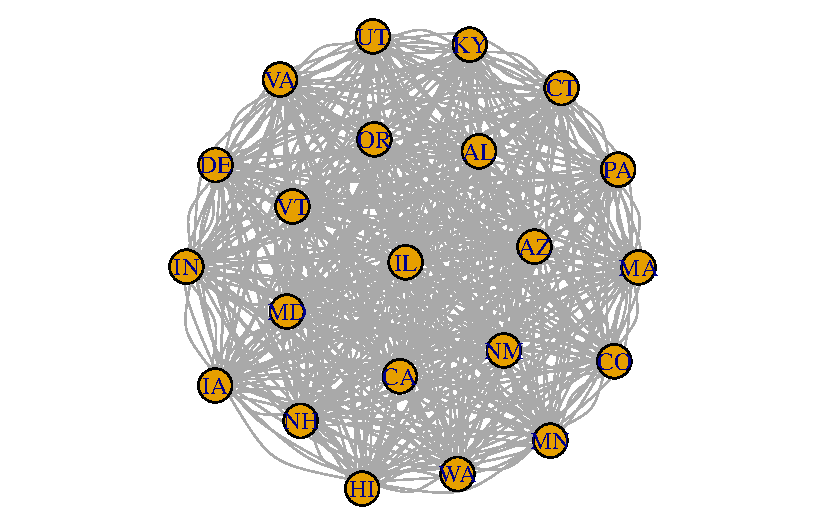
\includegraphics{state_dyadic_regression_files/figure-pdf/unnamed-chunk-4-1.pdf}

}

\end{figure}

\begin{Shaded}
\begin{Highlighting}[]
\CommentTok{\#plot(igraph, vertex.label = V(igraph)$state)}

\CommentTok{\#DV}
\NormalTok{similarity }\OtherTok{\textless{}{-}} \FunctionTok{as\_adjacency\_matrix}\NormalTok{(igraph, }\AttributeTok{attr=}\StringTok{"shared\_score"}\NormalTok{)}
\NormalTok{similarity }\OtherTok{\textless{}{-}} \FunctionTok{as.matrix}\NormalTok{(similarity)}

\CommentTok{\#IVs}
\NormalTok{topic\_tweets }\OtherTok{\textless{}{-}} \FunctionTok{as.matrix}\NormalTok{(}\FunctionTok{as\_adjacency\_matrix}\NormalTok{(igraph, }\AttributeTok{attr=}\StringTok{"dif\_topic\_ratio"}\NormalTok{))}
\NormalTok{pro\_tweets }\OtherTok{\textless{}{-}} \FunctionTok{as.matrix}\NormalTok{(}\FunctionTok{as\_adjacency\_matrix}\NormalTok{(igraph, }\AttributeTok{attr=}\StringTok{"dif\_pro\_ratio"}\NormalTok{))}
\NormalTok{contiguity }\OtherTok{\textless{}{-}} \FunctionTok{as\_adjacency\_matrix}\NormalTok{(igraph, }\AttributeTok{attr=}\StringTok{"contig"}\NormalTok{)}
\NormalTok{contiguity }\OtherTok{\textless{}{-}} \FunctionTok{as.matrix}\NormalTok{(contiguity)}
\NormalTok{ideology }\OtherTok{\textless{}{-}} \FunctionTok{as\_adjacency\_matrix}\NormalTok{(igraph, }\AttributeTok{attr=}\StringTok{"dif\_mrp\_ideology"}\NormalTok{)}
\NormalTok{ideology }\OtherTok{\textless{}{-}} \FunctionTok{as.matrix}\NormalTok{(ideology)}
\NormalTok{white }\OtherTok{\textless{}{-}} \FunctionTok{as\_adjacency\_matrix}\NormalTok{(igraph, }\AttributeTok{attr=}\StringTok{"dif\_white"}\NormalTok{)}
\NormalTok{white }\OtherTok{\textless{}{-}} \FunctionTok{as.matrix}\NormalTok{(white)}
\NormalTok{black }\OtherTok{\textless{}{-}} \FunctionTok{as\_adjacency\_matrix}\NormalTok{(igraph, }\AttributeTok{attr=}\StringTok{"dif\_black"}\NormalTok{)}
\NormalTok{black }\OtherTok{\textless{}{-}} \FunctionTok{as.matrix}\NormalTok{(black)}
\NormalTok{urban }\OtherTok{\textless{}{-}} \FunctionTok{as.matrix}\NormalTok{(}\FunctionTok{as\_adjacency\_matrix}\NormalTok{(igraph, }\AttributeTok{attr =} \StringTok{"dif\_urban\_index"}\NormalTok{))}
\NormalTok{income }\OtherTok{\textless{}{-}} \FunctionTok{as.matrix}\NormalTok{(}\FunctionTok{as\_adjacency\_matrix}\NormalTok{(igraph, }\AttributeTok{attr =} \StringTok{"dif\_med\_inc"}\NormalTok{))}
\CommentTok{\#other IVs}

\CommentTok{\#gov\_gender \textless{}{-} import(here("data/gov\_gender\_mat.Rds"))}
\CommentTok{\#gov\_age \textless{}{-} import(here("data/gov\_age\_mat.Rds"))}
\CommentTok{\#gov\_party \textless{}{-} import(here("data/gov\_party\_mat.Rds"))}

\NormalTok{topic\_matrices }\OtherTok{\textless{}{-}} \FunctionTok{array}\NormalTok{(}\ConstantTok{NA}\NormalTok{, }\FunctionTok{c}\NormalTok{(}\DecValTok{7}\NormalTok{, }\FunctionTok{length}\NormalTok{(contiguity[}\DecValTok{1}\NormalTok{,]),}\FunctionTok{length}\NormalTok{(contiguity[}\DecValTok{1}\NormalTok{,]))) }


\NormalTok{topic\_matrices[}\DecValTok{1}\NormalTok{,,] }\OtherTok{\textless{}{-}}\NormalTok{ contiguity}
\NormalTok{topic\_matrices[}\DecValTok{2}\NormalTok{,,] }\OtherTok{\textless{}{-}}\NormalTok{ ideology}
\NormalTok{topic\_matrices[}\DecValTok{3}\NormalTok{,,] }\OtherTok{\textless{}{-}}\NormalTok{ white}
\NormalTok{topic\_matrices[}\DecValTok{4}\NormalTok{,,] }\OtherTok{\textless{}{-}}\NormalTok{ black}
\NormalTok{topic\_matrices[}\DecValTok{5}\NormalTok{,,] }\OtherTok{\textless{}{-}}\NormalTok{ topic\_tweets}
\NormalTok{topic\_matrices[}\DecValTok{6}\NormalTok{,,] }\OtherTok{\textless{}{-}}\NormalTok{ urban}
\NormalTok{topic\_matrices[}\DecValTok{7}\NormalTok{,,] }\OtherTok{\textless{}{-}}\NormalTok{ income}
\CommentTok{\# state\_matrices[8,,] \textless{}{-} gov\_gender}
\CommentTok{\# state\_matrices[9,,] \textless{}{-} gov\_age}
\CommentTok{\# state\_matrices[10,,] \textless{}{-} gov\_party}

\NormalTok{pro\_matrices }\OtherTok{\textless{}{-}} \FunctionTok{array}\NormalTok{(}\ConstantTok{NA}\NormalTok{, }\FunctionTok{c}\NormalTok{(}\DecValTok{7}\NormalTok{, }\FunctionTok{length}\NormalTok{(contiguity[}\DecValTok{1}\NormalTok{,]),}\FunctionTok{length}\NormalTok{(contiguity[}\DecValTok{1}\NormalTok{,]))) }


\NormalTok{pro\_matrices[}\DecValTok{1}\NormalTok{,,] }\OtherTok{\textless{}{-}}\NormalTok{ contiguity}
\NormalTok{pro\_matrices[}\DecValTok{2}\NormalTok{,,] }\OtherTok{\textless{}{-}}\NormalTok{ ideology}
\NormalTok{pro\_matrices[}\DecValTok{3}\NormalTok{,,] }\OtherTok{\textless{}{-}}\NormalTok{ white}
\NormalTok{pro\_matrices[}\DecValTok{4}\NormalTok{,,] }\OtherTok{\textless{}{-}}\NormalTok{ black}
\NormalTok{pro\_matrices[}\DecValTok{5}\NormalTok{,,] }\OtherTok{\textless{}{-}}\NormalTok{ pro\_tweets}
\NormalTok{pro\_matrices[}\DecValTok{6}\NormalTok{,,] }\OtherTok{\textless{}{-}}\NormalTok{ urban}
\NormalTok{pro\_matrices[}\DecValTok{7}\NormalTok{,,] }\OtherTok{\textless{}{-}}\NormalTok{ income}
\end{Highlighting}
\end{Shaded}

Run regression

\begin{Shaded}
\begin{Highlighting}[]
\CommentTok{\#library(statnet)}
\CommentTok{\#detach(package:igraph,unload=TRUE)}

\CommentTok{\#first run network regression on topic ratio difference}
\NormalTok{state\_sim\_lm }\OtherTok{\textless{}{-}}\NormalTok{ sna}\SpecialCharTok{::}\FunctionTok{netlm}\NormalTok{(similarity, topic\_matrices, }\AttributeTok{reps=}\DecValTok{1000}\NormalTok{)}

\NormalTok{state\_model }\OtherTok{\textless{}{-}} \FunctionTok{list}\NormalTok{()}
\NormalTok{state\_model }\OtherTok{\textless{}{-}} \FunctionTok{summary}\NormalTok{(state\_sim\_lm)}

\NormalTok{state\_model}\SpecialCharTok{$}\NormalTok{names }\OtherTok{\textless{}{-}} \FunctionTok{c}\NormalTok{(}\StringTok{"Intercept"}\NormalTok{, }\StringTok{"Contiguity"}\NormalTok{, }\StringTok{"Ideology"}\NormalTok{, }\StringTok{"White"}\NormalTok{, }\StringTok{"Black"}\NormalTok{, }\StringTok{"BLM related tweets"}\NormalTok{, }\StringTok{"Urban"}\NormalTok{, }\StringTok{"Income"}\NormalTok{)}


\NormalTok{state\_model}\SpecialCharTok{$}\NormalTok{coefficients }\OtherTok{=} \FunctionTok{round}\NormalTok{(state\_model}\SpecialCharTok{$}\NormalTok{coefficients, }\DecValTok{2}\NormalTok{)}
\NormalTok{state\_model}
\end{Highlighting}
\end{Shaded}

\begin{verbatim}

OLS Network Model

Residuals:
        0%        25%        50%        75%       100% 
-5.9101554 -2.2916648 -0.5753836  1.7820792 11.0792205 

Coefficients:
                   Estimate Pr(<=b) Pr(>=b) Pr(>=|b|)
Intercept           5.25    1.000   0.000   0.000    
Contiguity         -0.15    0.318   0.682   0.648    
Ideology           -1.70    0.175   0.825   0.380    
White              -3.26    0.057   0.943   0.095    
Black               0.62    0.525   0.475   0.864    
BLM related tweets 15.21    0.942   0.058   0.153    
Urban               0.26    0.811   0.189   0.387    
Income              0.00    0.011   0.989   0.017    

Residual standard error: 3.427 on 454 degrees of freedom
Multiple R-squared: 0.1941  Adjusted R-squared: 0.1817 
F-statistic: 15.62 on 7 and 454 degrees of freedom, p-value:     0 


Test Diagnostics:

    Null Hypothesis: qap 
    Replications: 1000 
    Coefficient Distribution Summary:

        Intercept Contiguity   Ideology      White      Black
Min     -6.395639  -3.377815  -7.325313 -11.001664 -12.976956
1stQ    -0.718206  -0.799633  -1.422376  -2.778180  -1.803581
Median   0.991335   0.032467   0.118207   0.361599   0.344762
Mean     1.031102   0.012854   0.080057   0.027649   0.079611
3rdQ     2.694251   0.802425   1.745521   2.742344   2.245808
Max      9.962641   4.575269   6.985654   7.781032   7.947339
       BLM related tweets      Urban     Income
Min            -11.632248  -8.907407  -7.818874
1stQ            -2.156872  -1.669418  -1.921779
Median           0.127055  -0.005902   0.102728
Mean            -0.181745  -0.075501   0.019481
3rdQ             1.985030   1.596607   1.936870
Max              7.912087   7.088222   7.445831
\end{verbatim}

\begin{Shaded}
\begin{Highlighting}[]
\CommentTok{\#second regression on pro blm ratio difference}
\NormalTok{state\_sim\_lm }\OtherTok{\textless{}{-}}\NormalTok{ sna}\SpecialCharTok{::}\FunctionTok{netlm}\NormalTok{(similarity, pro\_matrices, }\AttributeTok{reps=}\DecValTok{1000}\NormalTok{)}

\NormalTok{state\_model }\OtherTok{\textless{}{-}} \FunctionTok{list}\NormalTok{()}
\NormalTok{state\_model }\OtherTok{\textless{}{-}} \FunctionTok{summary}\NormalTok{(state\_sim\_lm)}

\NormalTok{state\_model}\SpecialCharTok{$}\NormalTok{names }\OtherTok{\textless{}{-}} \FunctionTok{c}\NormalTok{(}\StringTok{"Intercept"}\NormalTok{, }\StringTok{"Contiguity"}\NormalTok{, }\StringTok{"Ideology"}\NormalTok{, }\StringTok{"White"}\NormalTok{, }\StringTok{"Black"}\NormalTok{, }\StringTok{"Pro BLM tweets"}\NormalTok{, }\StringTok{"Urban"}\NormalTok{, }\StringTok{"Income"}\NormalTok{)}
\NormalTok{state\_model}\SpecialCharTok{$}\NormalTok{coefficients }\OtherTok{=} \FunctionTok{round}\NormalTok{(state\_model}\SpecialCharTok{$}\NormalTok{coefficients, }\DecValTok{2}\NormalTok{)}
\NormalTok{state\_model}
\end{Highlighting}
\end{Shaded}

\begin{verbatim}

OLS Network Model

Residuals:
        0%        25%        50%        75%       100% 
-5.9314705 -2.3432386 -0.3885335  1.8426697 10.9741785 

Coefficients:
               Estimate Pr(<=b) Pr(>=b) Pr(>=|b|)
Intercept       5.38    1.000   0.000   0.000    
Contiguity     -0.38    0.140   0.860   0.275    
Ideology       -2.08    0.112   0.888   0.231    
White          -2.96    0.104   0.896   0.133    
Black           0.03    0.476   0.524   0.994    
Pro BLM tweets 60.52    0.987   0.013   0.055    
Urban           0.17    0.699   0.301   0.594    
Income          0.00    0.006   0.994   0.008    

Residual standard error: 3.405 on 454 degrees of freedom
Multiple R-squared: 0.2042  Adjusted R-squared: 0.1919 
F-statistic: 16.64 on 7 and 454 degrees of freedom, p-value:     0 


Test Diagnostics:

    Null Hypothesis: qap 
    Replications: 1000 
    Coefficient Distribution Summary:

        Intercept Contiguity   Ideology      White      Black Pro BLM tweets
Min     -7.064152  -3.442074  -6.902859  -9.327602 -12.072480     -11.046328
1stQ    -0.443409  -0.937397  -1.357975  -2.561132  -1.776194      -2.078293
Median   1.358349  -0.040363   0.079141   0.288398   0.210415       0.347958
Mean     1.366615  -0.022650   0.022952  -0.154449   0.001613      -0.030196
3rdQ     3.112687   0.821949   1.462865   2.644901   2.106937       2.025831
Max      9.487554   6.888411   5.245616   8.048107   7.277918       6.571469
            Urban     Income
Min     -8.252359  -7.021739
1stQ    -1.734432  -1.666948
Median   0.099520   0.138524
Mean    -0.090373   0.066930
3rdQ     1.735252   1.795810
Max      6.319648   6.077705
\end{verbatim}

\begin{Shaded}
\begin{Highlighting}[]
\CommentTok{\#nl\textless{}{-} sna::netlm(similarity,           \# Dependent variable/network}
\CommentTok{\#         list(contiguity, ideology, white, black, urban, income), \# List the independent variables/networks}
\CommentTok{\#          reps=1000) }
\end{Highlighting}
\end{Shaded}




\end{document}
